\section{Verifier-Constrained Code Generation}
\label{sec:codegen}

This section describes how \kunai lowers filter expressions over
nested encapsulation and variable-length structures into eBPF
bytecode accepted by the Linux verifier.

The challenge is that the location of a target field may depend on
packet contents and therefore be known only at run time. A naive
lowering produces packet accesses whose range the verifier cannot
prove and is therefore rejected. \kunai addresses this challenge
through two code-generation patterns: recorded-base addressing
(\S\ref{sec:offset}) and constant-bounded scanning
(\S\ref{sec:bounded}).

\subsection{Recording Header Start Offsets Explicitly}
\label{sec:offset}

\kunai records each header's start offset at run time and reads a
field as a relative offset from that start. Consider again the GTP-U
inner-IPv4 filter of \S\ref{sec:dsl}: \texttt{inner.dst} is not at a
fixed offset, since the start of the inner IPv4 changes with the outer
IPv4 length, the GTP optional fields, and the structure of the
encapsulation.

A fixed compile-time offset reads the wrong bytes whenever the
variable-length parts before the field are non-empty, so the offset
must be computed at run time. The verifier, however, cannot bound a
run-time offset against the native-XDP packet pointer
\texttt{PTR\_TO\_PACKET}, cannot prove the read stays within
\texttt{data\_end}, and rejects the bytecode.

\kunai detects this boundary at the resolve stage and marks every
layer after one with a variable-length layout as a run-time offset.
The generated eBPF bytecode then records each header's start offset
into a stack slot as it traverses the header at run time.
\figref{fig:layerstart} illustrates this offset recording and a
bounds-checked load that uses the recorded offset.

\begin{figure}[htbp]
  \centering
  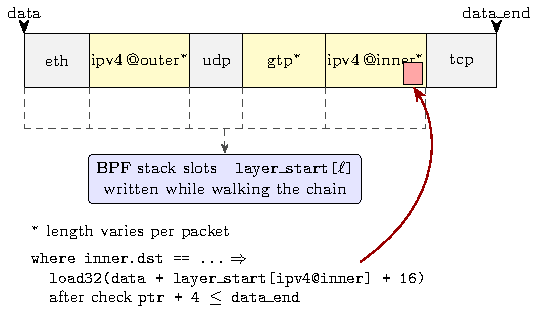
\includegraphics[width=\columnwidth]{figures/fig_layerstart.pdf}
  \caption{Recording each header's start offset into a stack slot, and
  reading \texttt{inner.dst} as a bounds-checked load at layer-start
  $+$ field offset.}
  \label{fig:layerstart}
\end{figure}

Every field access takes the same form: \kunai loads the layer's start
offset, adds the field offset and width, checks the access against
\texttt{data\_end}, loads, and compares. Because type-mismatched
comparisons and a \texttt{proto.field} reference under a repeated
protocol are already rejected at the analysis stage of
\S\ref{sec:overview}, code generation need only emit this bounds-checked
load, even for a chain whose subsequent-header start changes at run time.

\subsection{Lowering Variable-Length Structures to Bounded Bytecode}
\label{sec:bounded}

Because the element count or the length of each element changes per
packet, variable-length structures such as SRv6 segments and TCP
options cannot be walked at a fixed offset. \kunai puts the walk into a
verifier-accepted form by translating it into bytecode with a
compile-time constant bound.

\kunai generates the walk as one of two kinds of bytecode, chosen by
the bound and applied uniformly to chain quantifiers and
\texttt{any()}/\texttt{all()} aux-list walks. A small compile-time bound
within a fixed threshold is unrolled in place. A larger or unbounded one
is lowered to a
\texttt{bpf\_loop} callback with a constant
bound~\cite{bpf_loop_helper}, whose size no longer grows with the
bound. This case covers a parser-machine self-loop, an unbounded chain
quantifier, and a chain or aux-list walk past the threshold.

Algorithm~\ref{alg:walk} gives the shared skeleton. The two lowerings
below fill in its \textsc{stop}, \textsc{stride}, and \textsc{step}
steps, each emitted by its own generator.

\begin{algorithm}[htbp]
  \caption{Bounded walk skeleton; \textsc{stop}, \textsc{stride}, and
  \textsc{step} are filled in per structure.}
  \label{alg:walk}
  \begin{algorithmic}[1]
    \Require $data,\ data\_end,\ base,\ cap$; \textsc{stop}, \textsc{stride}, \textsc{step} per structure
    \State $r \gets \bot$;\ $off \gets base$
    \For{$i \gets 0$ \textbf{to} $cap-1$} \Comment{$cap$: compile-time bound}
      \State \textbf{if} $\textsc{stop}(i, off)$ \textbf{then break} \Comment{count reached, or end/END/malformed}
      \State $ptr \gets data + off$
      \State \textbf{if} $ptr + w > data\_end$ \textbf{then break} \Comment{$w$: bytes read; bounds check}
      \State $r \gets \textsc{step}(ptr)$; \textbf{break if} $r$ decides \Comment{compare, or record option}
      \State $off \gets off + \textsc{stride}(ptr)$ \Comment{constant, or this option's length}
    \EndFor
    \State \Return $r$
  \end{algorithmic}
\end{algorithm}

\kunai fills in this skeleton in two ways, chosen by the structure
rather than the protocol. The compiler classifies each parser loop by
the shape of its states when it loads the protocol definition. A
chain walk over stacked headers such as MPLS needs no loop
classification, since the protocol definition declares the
bottom-of-stack sentinel as a chain-end constant and the quantifier
bound caps the walk. A loop qualifies as a counted aux-list walk
when it extracts elements with \texttt{pkt.extract(stack.next)} under
a \texttt{ParserCounter} seeded from a whole-byte header field and
decremented once per element, so the seed field gives the run-time
count, as \texttt{last\_entry + 1} does for SRv6 in
\figref{fig:p4srv6}. It qualifies as a TLV self-loop when its
\texttt{select} dispatches on a \texttt{lookahead} of the kind byte,
optionally with a byte-count counter as in IPv4 options and Geneve.
The compiler rejects a multi-state parser cycle matching
neither shape at load time rather than compiling it to a wrong walk.

A \emph{counted aux-list walk} handles a list
of fixed-size elements with a run-time count, such as the SRv6 segment
list: \textsc{stop} is $i \geq count$, \textsc{stride} is the constant
element width, and \textsc{step} compares the element field to the
target and decides the walk on a match. For the SRv6 segment filter of
\S\ref{sec:dsl}, \texttt{base = srh\_start + SRH\_FIXED\_SIZE},
\texttt{stride = width = 16}, \texttt{count = last\_entry + 1} (the SRv6
parser's segment-walk seed in \S\ref{sec:p4subset}), and
\texttt{target = fc00::1}.

A \emph{TLV self-loop} handles options that differ in kind and length,
such as TCP options, where a reference like
\texttt{tcp.\allowbreak options.\allowbreak MSS.\allowbreak value} sits
at no fixed offset. Here \textsc{stride} is each option's length,
read at the cursor; \textsc{stop} fires when the cursor reaches the end
of the options, on an END option, on a malformed option (\texttt{len < 2}
or \texttt{cursor + len > options\_end}), or at the iteration bound; and
\textsc{step} dispatches on the option kind and records the position of
the referenced option, which the \texttt{where} clause then reads after
the walk. An option field is loaded only after checking that its option
header stays within the packet window.

In either instantiation, and in either the fixed-unrolling or the
\texttt{bpf\_loop} form, the bound is a compile-time constant and a
bounds check precedes every packet load. The verifier can therefore
confirm both the loop bound and the range of every packet access.

So that the generated bytecode is accepted across kernel versions,
\kunai avoids instructions available only on newer versions. For
byte-order conversion, for example, it uses the \texttt{BPF\_END}
instruction, available on older versions, rather than the
\texttt{BSWAP} instruction introduced in 6.6~\cite{bpf_isa,bpf_cpuv4}.

The building blocks behind these patterns are standard practice in
hand-written eBPF. Programmers routinely place a bounds check against
\texttt{data\_end} before each access and bound every loop by a
constant or by \texttt{bpf\_loop}. \kunai's contribution is not the
techniques but their systematic derivation. The compiler selects and
applies them from the resolved filter structure and protocol
definition, so a filter author writes none of them by hand. Because
\kunai selects the lowering from a structure's shape rather than its
protocol name, GTP-U, SRv6, Geneve, and TCP options need no
per-protocol code in the generator.
